\chapter{Bayesian quantile deep echo state networks for nonlinear time series}
\label{ch:research-c}

\begin{singlespace}
\noindent\textit{This chapter is based on joint work by Antonio de Leon, Raquel Prado, and Bruno Sans'o. The current corrected-v4 manuscript line supplies the chapter spine. The conditional-quantile target, central Q--DESN models, principal evidence, interpretation, and limitations remain in the chapter; complete posterior derivations, algorithms, secondary diagnostics, and supporting numerical results are retained in Appendix~\ref{app:qdesn-technical}.}
\end{singlespace}

\section{Chapter overview}
\noindent
Conditional quantiles are central to asymmetric decision losses, tail-risk
assessment, and interval forecasts, but Bayesian quantile regression for
nonlinear time series can be difficult when the temporal feature vector is
high-dimensional. We develop the quantile deep echo state network (Q--DESN), a
Bayesian quantile regression model conditional on fixed features generated by a
deep echo state network. Conditional on a specified reservoir construction and
feature map, posterior uncertainty is assigned to the regression coefficients,
likelihood, and shrinkage parameters.
Single-level fits use asymmetric Laplace or quantile-fixed generalized
asymmetric Laplace working likelihoods with ridge or regularized-horseshoe
priors. Posterior computation uses Markov chain Monte Carlo when computationally
practical and a model-specific variational Bayes approximation for analyses
requiring repeated fitting. For quantile grids, we compare
independent level-wise regressions followed by monotone rearrangement with a
joint quantile-vector regression that shrinks adjacent quantile-specific
coefficient differences. Synthetic studies, a single-origin retrospective
Global Flood Awareness System (GloFAS) streamflow case, and a region-frozen
PriceFM comparison show how performance varies with the data-generating
mechanism and evaluation design.
\newcommand{\GlofasApplicationCurrentRunId}{\detokenize{glofas_part4_joint_al_sweep10_20260911}}
\newcommand{\GlofasApplicationCurrentConfigPath}{\detokenize{tables/glofas_application_part4_model_spec__glofas_part4_joint_al_sweep10_20260911.csv}}
\newcommand{\GlofasApplicationCurrentPromotionManifest}{\detokenize{tables/glofas_application_part4_selection_decision__glofas_part4_joint_al_sweep10_20260911.csv}}
\newcommand{\GlofasApplicationCurrentSelectionManifest}{\detokenize{tables/glofas_application_part4_selection_decision__glofas_part4_joint_al_sweep10_20260911.csv}}
\newcommand{\GlofasApplicationCurrentCandidateId}{\detokenize{glofas_part4_joint_al_continuation_20260907}}
\newcommand{\GlofasApplicationCurrentDiscrepancyTransitionStrategy}{\detokenize{joint latent-path ensemble likelihood}}
\newcommand{\GlofasApplicationCurrentScoreTable}{tables/ch04-qdesn/glofas_application_part4_main_scores__glofas_part4_joint_al_sweep10_presentation_v2_20260911.tex}
\newcommand{\GlofasApplicationCurrentCorrectedPathsFigure}{figures/ch04-qdesn/glofas_application/glofas_part4_joint_al_last30_issued28__glofas_part4_joint_al_sweep10_presentation_v2_20260911.pdf}
\newcommand{\GlofasApplicationCurrentForecastWindowFigure}{figures/ch04-qdesn/glofas_application/glofas_part4_joint_al_last30_issued28__glofas_part4_joint_al_sweep10_presentation_v2_20260911.pdf}
\newcommand{\GlofasApplicationCurrentQdesnCheckLoss}{0.4180}
\newcommand{\GlofasApplicationCurrentRawCheckLoss}{0.7713}
\newcommand{\GlofasApplicationCurrentCheckLossReduction}{45.8\%}
\newcommand{\GlofasApplicationCurrentQdesnIntervalScore}{5.3889}
\newcommand{\GlofasApplicationCurrentRawIntervalScore}{24.5037}
\newcommand{\GlofasApplicationCurrentIntervalScoreReduction}{78.0\%}
\newcommand{\GlofasApplicationCurrentQdesnAcrps}{0.8374}
\newcommand{\GlofasApplicationCurrentRawAcrps}{1.4360}
\newcommand{\GlofasApplicationCurrentAcrpsReduction}{41.7\%}
\newcommand{\GlofasApplicationCurrentQdesnCrps}{0.8374}
\newcommand{\GlofasApplicationCurrentRawCrps}{1.4360}
\newcommand{\GlofasApplicationCurrentCrpsReduction}{41.7\%}
\newcommand{\GlofasApplicationCurrentQdesnMeanCoverage}{0.929}
\newcommand{\GlofasApplicationCurrentRawMeanCoverage}{0.000}
\newcommand{\GlofasApplicationCurrentScoredHorizons}{28}
\newcommand{\GlofasApplicationCurrentOriginDate}{2022-12-25}
\newcommand{\GlofasApplicationCurrentVbIterations}{10 joint outer iterations; cap reached after RHS release; all inner and RHS gates passed; strict outer tolerance not met}
\newcommand{\GlofasApplicationCurrentNumericalStatus}{\detokenize{cap-stabilized after RHS release; not strictly outer-converged}}
\newcommand{\GlofasApplicationCurrentReservoirDepth}{1}
\newcommand{\GlofasApplicationCurrentReservoirSize}{3000}
\newcommand{\GlofasApplicationCurrentReducerSize}{none}
\newcommand{\GlofasApplicationCurrentReservoirMemory}{360}
\newcommand{\GlofasApplicationCurrentReservoirWashout}{500}
\newcommand{\GlofasApplicationCurrentReservoirAlpha}{0.5}
\newcommand{\GlofasApplicationCurrentReservoirRho}{0.9}
\newcommand{\GlofasApplicationCurrentReservoirPiW}{0.03}
\newcommand{\GlofasApplicationCurrentReservoirPiIn}{1}
\newcommand{\GlofasApplicationCurrentReservoirWinScaleGlobal}{0.18}
\newcommand{\GlofasApplicationCurrentReservoirWinScaleBias}{0.18}
\newcommand{\GlofasApplicationCurrentReservoirSeed}{20260512}
\newcommand{\GlofasApplicationCurrentReferenceReservoirDepth}{1}
\newcommand{\GlofasApplicationCurrentReferenceReservoirSize}{3000}
\newcommand{\GlofasApplicationCurrentReferenceReducerSize}{none}
\newcommand{\GlofasApplicationCurrentReferenceReservoirMemory}{360}
\newcommand{\GlofasApplicationCurrentReferenceReservoirWashout}{500}
\newcommand{\GlofasApplicationCurrentReferenceReservoirAlpha}{0.5}
\newcommand{\GlofasApplicationCurrentReferenceReservoirRho}{0.9}
\newcommand{\GlofasApplicationCurrentReferenceReservoirPiW}{0.03}
\newcommand{\GlofasApplicationCurrentReferenceReservoirPiIn}{1}
\newcommand{\GlofasApplicationCurrentReferenceReservoirWinScaleGlobal}{0.18}
\newcommand{\GlofasApplicationCurrentReferenceReservoirWinScaleBias}{0.18}
\newcommand{\GlofasApplicationCurrentReferenceReservoirSeed}{20260512}
\newcommand{\GlofasApplicationCurrentDiscrepancyReservoirDepth}{1}
\newcommand{\GlofasApplicationCurrentDiscrepancyReservoirSize}{2500}
\newcommand{\GlofasApplicationCurrentDiscrepancyReservoirMemory}{360}
\newcommand{\GlofasApplicationCurrentDiscrepancyReservoirWashout}{500}
\newcommand{\GlofasApplicationCurrentDiscrepancyReservoirAlpha}{0.8}
\newcommand{\GlofasApplicationCurrentDiscrepancyReservoirRho}{0.7}
\newcommand{\GlofasApplicationCurrentDiscrepancyReservoirPiW}{0.03}
\newcommand{\GlofasApplicationCurrentDiscrepancyReservoirPiIn}{1}
\newcommand{\GlofasApplicationCurrentDiscrepancyReservoirWinScaleGlobal}{0.18}
\newcommand{\GlofasApplicationCurrentDiscrepancyReservoirWinScaleBias}{0.18}
\newcommand{\GlofasApplicationCurrentDiscrepancyReservoirSeed}{20261521}
\newcommand{\GlofasApplicationCurrentSharedRhsTau}{1}
\newcommand{\GlofasApplicationCurrentDiscrepancyRhsTau}{0.001}
\newcommand{\GlofasApplicationCurrentRhsTau}{1}
\newcommand{\GlofasApplicationCurrentSpreadCalibrationEnabled}{no}
\newcommand{\GlofasApplicationCurrentSpreadCalibrationFactor}{1.0}
\newcommand{\GlofasApplicationCurrentSpreadCalibrationAdditiveWidth}{0.0}
\newcommand{\GlofasApplicationCurrentSpreadCalibrationCenterQuantile}{0.50}
\newcommand{\GlofasApplicationCurrentSpreadCalibrationId}{\detokenize{none}}
\newcommand{\GlofasApplicationCurrentSpreadCalibrationDescription}{\detokenize{No spread calibration or crossing correction was applied.}}
\newcommand{\GlofasApplicationCurrentObservedHistoryAcrps}{0.0751}
\newcommand{\GlofasApplicationCurrentObservedHistoryCoverage}{0.920}
\newcommand{\GlofasApplicationCurrentObservedHistoryDates}{12,495}
\newcommand{\GlofasApplicationCurrentSupplementScoreTable}{tables/ch04-qdesn/glofas_application_part4_supplementary_scores__glofas_part4_joint_al_sweep10_presentation_v2_20260911.tex}
\newcommand{\GlofasApplicationCurrentNormalComparisonFigure}{figures/ch04-qdesn/glofas_application/diagnostics/glofas_part4_normal_comparison__glofas_part4_joint_al_sweep10_presentation_v2_20260911.pdf}
\newcommand{\GlofasApplicationCurrentIndependentComparisonFigure}{figures/ch04-qdesn/glofas_application/diagnostics/glofas_part4_independent_quantile_comparison__glofas_part4_joint_al_sweep10_presentation_v2_20260911.pdf}
\newcommand{\GlofasApplicationCurrentJointComparisonFigure}{figures/ch04-qdesn/glofas_application/diagnostics/glofas_part4_joint_quantile_comparison__glofas_part4_joint_al_sweep10_presentation_v2_20260911.pdf}
\newcommand{\GlofasApplicationCurrentHistoricalGuardrailTable}{tables/ch04-qdesn/glofas_application_part4_historical_guardrail__glofas_part4_joint_al_sweep10_presentation_v2_20260911.tex}


\newcommand{\PricefmFullRegionFolds}{114}
\newcommand{\PricefmFullRegions}{38}
\newcommand{\PricefmFullFolds}{3}
\newcommand{\PricefmFullQdesnWins}{54}
\newcommand{\PricefmFullPricefmWins}{60}
\newcommand{\PricefmFullQdesnWinRate}{47.4\%}
\newcommand{\PricefmCurrentRegionWins}{16}
\newcommand{\PricefmCurrentRegionLosses}{22}
\newcommand{\PricefmCurrentAlRegions}{11}
\newcommand{\PricefmCurrentExalRegions}{27}
\newcommand{\PricefmFullMeanQdesnAql}{7.217}
\newcommand{\PricefmFullMeanPricefmAql}{7.039}
\newcommand{\PricefmFullMeanDeltaAql}{+0.178}
\newcommand{\PricefmFullMedianDeltaAql}{+0.071}
\newcommand{\PricefmCurrentHistoricalAql}{6.824}
\newcommand{\PricefmFullPaperQuantiles}{0.10, 0.25, 0.45, 0.50, 0.55, 0.75, 0.90}
\newcommand{\PricefmCurrentMainSummaryTable}{tables/ch04-qdesn/pricefm_r98_main_aql_summary.tex}
\newcommand{\PricefmCurrentGlobalComparisonTable}{tables/ch04-qdesn/pricefm_r98_global_aql_comparison.tex}
\newcommand{\PricefmCurrentRegionFigure}{figures/ch04-qdesn/pricefm_application/pricefm_r98_region_aql_comparison.pdf}

% The source PDF uses an embedded Type 3 plot font. This derivative preserves
% the same vector display with the plot lettering converted to outlines so the
% dissertation PDF satisfies the embedded-font requirement.
\renewcommand{\PricefmCurrentRegionFigure}{figures/ch04-qdesn/pricefm_application/pricefm_r98_region_aql_comparison_fontsafe.pdf}

\section{Introduction}
\label{qdesn:sec:intro}

Conditional quantiles are natural summaries for asymmetric decision losses,
tail-risk assessment, and interval forecasts. If \(\mathcal F_t\) is the
information available at forecast origin \(t\), the level-\(p\) quantile of a
future response is
\[
Q_{t,h}(p)=\inf\{u:\Pr(Y_{t+h}\le u\mid\mathcal F_t)\ge p\},
\qquad 0<p<1.
\]
Quantile regression estimates this quantity directly
\citep{qdesn-KoenkerBassett1978,qdesn-Koenker2005}. Dynamic applications are more
difficult when nonlinear temporal structure must be represented by a large
number of correlated predictors and inference must be repeated over forecast
origins or probability levels.

Echo state networks (ESNs) represent temporal dependence through recurrent
nonlinear states whose reservoir weights are drawn once rather than estimated
with the regression coefficients
\citep{qdesn-Jaeger2001EchoState,qdesn-LukoseviciusJaeger2009ReservoirComputing}. Deep ESNs
stack these reservoirs to obtain features at several time scales
\citep{qdesn-GallicchioMicheliPedrelli2018DeepESNDesign}. We use the resulting states
as a fixed nonlinear design and place Bayesian quantile regression on the final
linear predictor. This separation retains the computational economy of
reservoir methods while providing regularized posterior inference for the
conditional quantile.

The proposed quantile deep echo state network (Q--DESN) uses either the
asymmetric Laplace (AL) likelihood or the quantile-fixed generalized
asymmetric Laplace likelihood of \citet{exd-yan2025family}, abbreviated exAL. Both are
working likelihoods: they define posterior inference for quantile-regression
parameters without asserting the corresponding error law
\citep{env-sriram2013theoretical,qdesn-YangWangHe2016ALInference,qdesn-JiLeeRabeHesketh2025ValidSE}.
The exAL family adds a shape parameter while preserving the chosen conditional
quantile as its location. Ridge regularization supplies a dense baseline, and
the regularized horseshoe (RHS) supplies adaptive global--local shrinkage with
a finite slab \citep{qdesn-CarvalhoPolsonScott2010HS,qdesn-PiironenVehtari2017RHS}.

Several ESN methods already address probabilistic or quantile forecasting
\citep{qdesn-McDermottWikle2018DeepESNUQ,qdesn-LvZhaoLiuWang2016QRESNE,qdesn-BonasWikleCastruccio2024CalibratedDeepESN}. Q--DESN differs by treating a
specified DESN realization as a fixed feature map and assigning a posterior to
the quantile-specific regression, likelihood, and shrinkage parameters. Its
linear dynamic comparators are the DQLM and exDQLM
\citep{env-goncalves,exd-me}, implemented in
version 1.1.1 of the CRAN package \pkg{exdqlm} \citep{qdesn-exdqlmRPackage}.

For a grid of probability levels, we distinguish two inferential strategies.
Independent regressions may be rearranged after fitting to obtain an ordered
reported grid \citep{qdesn-BarlowBrunk1972IsotonicDual,exd-chernozhukov2010}. A joint
quantile-vector regression instead shares information during estimation by
placing RHS priors on adjacent quantile-specific coefficient differences,
adapting the Quantile-Varying Parameter construction of
\citet{qdesn-KohnsSzendrei2025QVP}. This prior can reduce crossings but does not
enforce noncrossing; an ordered parameterization or explicit rearrangement is
still required for exact monotonicity
\citep{qdesn-WuLiu2009StepwiseNCQR,qdesn-BondellReichWang2010NoncrossingQR,qdesn-YangTokdar2017JointQuantilePlanes}.

This chapter develops the fixed-feature Bayesian Q--DESN formulation, its
independent and joint quantile-grid variants, and posterior computation by
Markov chain Monte Carlo (MCMC) and a model-specific variational Bayes
approximation. A single-quantile simulation compares Q--DESN with DQLM and
exDQLM; a second simulation isolates joint versus independent estimation of a
seven-level quantile grid. Retrospective GloFAS streamflow and PriceFM
electricity-price examples assess independent Q--DESN regressions under their
stated information sets. Appendix~\ref{app:qdesn-technical} contains the
complete posterior derivations, initialization and forecast details, secondary
diagnostics, and supporting numerical results needed to audit these
comparisons.

The presentation begins with reservoir construction and the conditional
quantile target, followed by the working-likelihood and prior specification.
The exact Gaussian readout then serves as a mean-regression baseline and an
initialization device before the MCMC and variational calculations. Simulation
evidence precedes the two retrospective applications so that the empirical
claims remain tied to their respective evaluation designs.

% ============================================================

% Restrained print palette and TikZ styles for the initialization diagram.
% Model families are identified by text and position in addition to color.
\definecolor{qiText}{HTML}{202124}
\definecolor{qiLine}{HTML}{62676C}
\definecolor{qiGaussian}{HTML}{737A80}
\definecolor{qiAL}{HTML}{31566D}
\definecolor{qiExAL}{HTML}{70444B}
\tikzset{
  qi/base/.style={rectangle,rounded corners=0pt,draw=qiLine,
    fill=white,text=qiText,line width=0.55pt,align=center,
    font=\normalfont\rmfamily\fontsize{9.5}{11}\selectfont,
    inner xsep=2.5pt,inner ysep=3pt,outer sep=0.3pt,
    minimum height=10mm},
  qi/gaussian/.style={qi/base,draw=qiGaussian},
  qi/al/.style={qi/base,draw=qiAL},
  qi/exal/.style={qi/base,draw=qiExAL},
  qi/heading/.style={text=qiText,align=left,inner sep=0pt,
    font=\normalfont\rmfamily\bfseries\fontsize{10}{11.5}\selectfont},
  qi/note/.style={text=qiText,align=left,inner sep=0pt,
    font=\normalfont\rmfamily\fontsize{9}{10.5}\selectfont},
  qi/dots/.style={inner sep=0.4pt,text=qiText,
    font=\normalfont\rmfamily\fontsize{9.5}{11}\selectfont},
  qi/arrow/.style={draw=qiLine,line width=0.55pt,
    -{Latex[length=1.65mm,width=1.12mm]},
    shorten <=0.35pt,shorten >=0.35pt},
  qi/collection/.style={draw=qiLine,line width=0.55pt},
  qi/comparison/.style={qi/arrow,dash pattern=on 2.5pt off 1.8pt}
}


\section{Reservoir specification, selection, and diagnostics}
\label{qdesn:sec:supp_reservoir_diagnostics}

Table~\ref{qdesn:tab:supp-reservoir-selection} summarizes the reservoir-design
quantities and their associated diagnostics. Posterior inference conditions on
the resulting feature map and quantifies uncertainty in the regression,
likelihood, and shrinkage parameters.

\begin{table}[!htbp]
\centering
\begingroup
\CompactTableStyle
\begin{tabularx}{\textwidth}{@{}>{\raggedright\arraybackslash}p{0.16\textwidth}
>{\raggedright\arraybackslash}p{0.25\textwidth}
>{\raggedright\arraybackslash}p{0.28\textwidth}
>{\raggedright\arraybackslash}X@{}}
\toprule
Component & Role in the fixed feature map & Design consideration & Potential concern \\
\midrule
\(D\) & Number of reservoir layers and hierarchy of time scales &
Evaluate a small prespecified set and retain additional depth only when
validation forecast criteria improve consistently across reservoir realizations. &
Unnecessary depth can add numerically unstable or redundant design columns. \\
\(\{n_d\},\{\tilde n_d\}\) & Number of reservoir states and lower-layer feature
dimension & Treat as the main complexity control, with reduction sizes chosen
as part of the same feature map. &
A large design relative to the sample size can yield weakly identified
coefficients or a poorly conditioned regression; redundant states can reduce
the effective rank of \(\mat X\). \\
\(m\) & Explicit lag memory entering the reservoir input & Choose a
domain-informed grid and require all lags to be available at the forecast
origin. & Excessive lags increase dimension and can incorporate observations
unavailable at the forecast origin if alignment is incorrect. \\
\(\{\alpha_d\},\{\rho_d\}\) & Reservoir time scale, persistence, and stability &
Compare jointly because both affect memory. Near-one radii require empirical
stability checks. & States concentrated near the activation bounds,
near-constant states, or sensitivity to initial conditions. \\
\(\{\pi^{(W)}_d\},\{\pi^{(\mathrm{in})}_d\}\) and input scaling & Recurrent
connectivity and input-induced variation & Fix from a small set of literature-guided
defaults; broaden the comparison when diagnostics show weak state variation or
concentration near the activation bounds. & Low connectivity can produce weakly
varying states; high connectivity or input scaling can concentrate states near
the activation bounds. \\
\(f,k,T_0\) & Nonlinearity, transformation of reduced lower-layer states, and initial-condition
washout & Fix before feature-map comparison, with \(T_0\) chosen relative to the
memory scale. & Short washout can leave initial-condition artifacts. \\
Random reservoir realization & Realization of the random feature map & Assess
variation across repeated reservoir realizations. &
Held-out scores can vary materially across realizations. \\
\bottomrule
\end{tabularx}
\endgroup
\caption{Reservoir specification and diagnostics for the fixed
Q--DESN feature map.}
\label{qdesn:tab:supp-reservoir-selection}
\end{table}

\subsection{Validation-based selection and initialization}
\label{qdesn:sec:supp_selection_initialization}

For a fixed statistical specification \(M\), reservoir candidates
\(R_j\) are compared on the designated validation observations using
the criterion stated for the analysis. The response convention, information
set, design rows, transformations, feature ordering, scaling quantities, and
forecast definition are held common across candidates. Reservoir states are
also checked for finite values, concentration near the activation bounds,
near-constant columns, and severe numerical dependence. The selected
specification satisfies
\[
\widehat R_M
\in
\argmin_{R_j:\,j=1,\ldots,J}
S_{\mathrm{val}}(R_j;M).
\]
The selected \(\widehat R_M\) is held fixed for
evaluation.

Suppose that the probability grid satisfies
\(p_1<\cdots<p_m=0.50<\cdots<p_K\).
After the Gaussian ridge and Gaussian \(\RHS\)--VB fits, compatible estimates
from the latter initialize the median AL regression. The lower side of the AL
grid is fitted in the order
\[
0.50\ \longrightarrow\ p_{m-1}\ \longrightarrow\ \cdots\
\longrightarrow\ p_1,
\]
and the upper side is fitted in the order
\[
0.50\ \longrightarrow\ p_{m+1}\ \longrightarrow\ \cdots\
\longrightarrow\ p_K.
\]
Thus each AL regression is initialized from the nearest completed level on the
same side of the median. For every \(k=1,\ldots,K\), the completed AL fit at
\(p_k\) initializes the exAL fit at \(p_k\). The exAL regressions may
therefore be fitted as soon as their matching AL fits are available.

The joint AL regression is initialized from the complete collection of
independent AL fits, and the joint exAL regression is initialized from the
complete collection of independent exAL fits. Let
\(\widehat\beta_{0k}^{\,\mathrm{ind}}\) and
\(\widehat{\vect\beta}_k^{\,\mathrm{ind}}\) denote the independent
intercept and slope estimates from the matching likelihood family. Initial
values for the level-specific joint coefficients are
\[
\beta_{0k}^{(0)}
=\widehat\beta_{0k}^{\,\mathrm{ind}},
\qquad
\vect\beta_k^{(0)}
=\widehat{\vect\beta}_k^{\,\mathrm{ind}},
\qquad k=1,\ldots,K.
\]
Under the adjacent-difference parameterization in
Section~\ref{qdesn:sec:joint_qdesn_supp}, the corresponding initial differences are
\begin{equation}
\vect\Delta_k^{(0)}
=\widehat{\vect\beta}_k^{\,\mathrm{ind}}
-\widehat{\vect\beta}_{k-1}^{\,\mathrm{ind}},
\qquad k=2,\ldots,K.
\label{qdesn:eq:supp-joint-initial-differences}
\end{equation}
Independent AL estimates are used for joint AL, and independent exAL estimates
are used for joint exAL in Eq.~\eqref{qdesn:eq:supp-joint-initial-differences}.

When the source and destination models differ, only parameters with
corresponding interpretations are used to construct starting values. Gaussian
residual scale and AL or exAL scale have different parameterizations, so the
initial value of the destination scale is obtained under its own
parameterization. Parameters specific to the exAL likelihood or coefficient
prior are initialized within their respective supports. For a VB-to-MCMC
initialization, the response, data period, design matrix, feature ordering,
transformations, reservoir realization, likelihood, probability level or grid,
parameterization, and prior specification agree. MCMC then targets the
posterior distribution of that same model. Convergence is assessed using the
diagnostics stated for the empirical analysis.

\begin{figure}[p]
  \centering
  \resizebox{\textwidth}{!}{% All coordinates are in millimetres. No scaling or clipping is used.
\begin{tikzpicture}[x=1mm,y=1mm]
  \node[qi/heading,anchor=west] at (0,0) {Preliminary Gaussian regressions};
  \node[qi/gaussian,minimum width=35mm] (ridge) at (17.5,-11)
    {Gaussian ridge\\regression};
  \node[qi/gaussian,minimum width=42mm] (rhs) at (62,-11)
    {Gaussian regression\\with \RHS{} prior (VB)};
  \draw[qi/arrow] (ridge.east) -- (rhs.west);

  \node[qi/heading,anchor=west] at (0,-24)
    {Independent quantile regressions};
  \node[qi/note,anchor=west] at (0,-29) {Variational fits};
  \node[qi/note,anchor=west] at (98,-11)
    {$p_1<\cdots<p_m=0.50<\cdots<p_K$};
  \node[qi/heading,align=center] at (146,-26.5)
    {Joint quantile\\regressions};

  \node[qi/al,minimum width=16mm] (al1) at (8,-40)
    {$\AL(p_1)$};
  \node[qi/al,minimum width=20mm] (allo) at (37,-40)
    {$\AL(p_{m-1})$};
  \node[qi/al,minimum width=19mm] (almed) at (62,-40)
    {$\AL(0.50)$\\median};
  \node[qi/al,minimum width=20mm] (alhi) at (87,-40)
    {$\AL(p_{m+1})$};
  \node[qi/al,minimum width=16mm] (alK) at (116,-40)
    {$\AL(p_K)$};
  \node[qi/dots] (aldotslo) at (21.5,-40) {$\cdots$};
  \node[qi/dots] (aldotshi) at (102.5,-40) {$\cdots$};
  \draw[qi/arrow] (rhs.south) -- (almed.north);
  \draw[qi/arrow] (almed.west) -- (allo.east);
  \draw[qi/arrow] (allo.west) -- (aldotslo.east);
  \draw[qi/arrow] (aldotslo.west) -- (al1.east);
  \draw[qi/arrow] (almed.east) -- (alhi.west);
  \draw[qi/arrow] (alhi.east) -- (aldotshi.west);
  \draw[qi/arrow] (aldotshi.east) -- (alK.west);

  \node[qi/exal,minimum width=16mm] (ex1) at (8,-64)
    {$\exAL(p_1)$};
  \node[qi/exal,minimum width=20mm] (exlo) at (37,-64)
    {$\exAL(p_{m-1})$};
  \node[qi/exal,minimum width=19mm] (exmed) at (62,-64)
    {$\exAL(0.50)$};
  \node[qi/exal,minimum width=20mm] (exhi) at (87,-64)
    {$\exAL(p_{m+1})$};
  \node[qi/exal,minimum width=16mm] (exK) at (116,-64)
    {$\exAL(p_K)$};
  \node[qi/dots] at (21.5,-64) {$\cdots$};
  \node[qi/dots] at (102.5,-64) {$\cdots$};
  \foreach \a/\b in {al1/ex1,allo/exlo,almed/exmed,alhi/exhi,alK/exK}
    \draw[qi/arrow] (\a.south) -- (\b.north);

  \draw[qi/collection] (124.8,-34.3) -- (127,-34.3)
    -- (127,-45.7) -- (124.8,-45.7);
  \draw[qi/collection] (124.8,-58.3) -- (127,-58.3)
    -- (127,-69.7) -- (124.8,-69.7);
  \node[qi/al,minimum width=25mm] (jointal) at (146,-40)
    {Joint AL\\regression (VB)};
  \node[qi/exal,minimum width=25mm] (jointex) at (146,-64)
    {Joint exAL\\regression (VB)};
  \draw[qi/arrow] (127,-40) -- (jointal.west);
  \draw[qi/arrow] (127,-64) -- (jointex.west);
  \node[qi/note,align=center] at (145,-49) {complete AL grid};
  \node[qi/note,align=center] at (145,-73) {complete exAL grid};

  \draw[draw=qiGaussian,line width=0.35pt] (0,-80) -- (159,-80);
  \node[qi/heading,anchor=west] at (0,-87) {Posterior simulation};
  \node[qi/heading,anchor=west] at (82,-87) {Model comparison};
  \node[qi/base,minimum width=29mm] (vb) at (14.5,-98)
    {VB fit\\of model $M$};
  \node[qi/base,minimum width=31mm] (mcmc) at (59,-98)
    {MCMC for the\\same model $M$};
  \draw[qi/arrow] (vb.east) -- (mcmc.west);
  \node[qi/note,anchor=north,align=center] at (36.5,-106)
    {same statistical specification};
  \node[qi/base,minimum width=33mm] (candidates) at (99,-98)
    {Fitted candidate\\specifications};
  \node[qi/base,minimum width=37mm] (criterion) at (140.5,-98)
    {Prespecified\\validation criterion};
  \draw[qi/comparison] (candidates.east) -- (criterion.west);
  \node[qi/note,anchor=north,align=center] at (120,-106)
    {comparison after fitting};
\end{tikzpicture}
}
  \caption[Sequential initialization centered at the median]{%
    Sequential initialization centered at the median for a probability grid that
contains 0.50. A Gaussian ridge regression initializes a Gaussian regression
with a regularized-horseshoe (RHS) prior fitted by variational Bayes (VB), and
compatible estimates from that fit supply starting values for the median
asymmetric Laplace (AL) regression. Independent AL regressions are then
initialized successively
from the nearest completed level on either side of 0.50. Each AL fit initializes
the extended asymmetric Laplace (exAL) regression at the matching probability
level. The complete independent AL and exAL grids initialize their respective
joint regressions. For a given statistical model, its VB fit supplies starting
values for Markov chain Monte Carlo (MCMC). Solid arrows denote initialization;
the dashed arrow denotes comparison using the prespecified validation
criterion. The joint simulation and the GloFAS and PriceFM analyses use this
initialization procedure; the independent validation study uses a separate
procedure. Here
exAL refers to the quantile-fixed generalized asymmetric Laplace working
likelihood.
%
  }
  \figalt{A Gaussian ridge regression initializes a Gaussian regularized-horseshoe
  variational fit, which initializes the median AL regression. Independent AL
  fits then proceed outward toward both tails; each initializes the exAL fit at
  the same probability level. Complete independent grids initialize the
  corresponding joint models, and fitted variational models initialize MCMC.}
  \label{qdesn:fig:supp-quantile-sequential-initialization}
\end{figure}

\section{Q--DESN formulation}
\label{qdesn:sec:model}

\subsection{Deep echo state network features}

Let \(\vect u_t=(y_{t-1},\ldots,y_{t-m},\vect z_t^\top)^\top\) contain response
lags and exogenous variables. For layer \(d\), \(\bar{\mat W}_d\) is a fixed
sparse recurrent matrix scaled to target spectral radius \(\rho_d\),
\(\mat W_d^{\mathrm{in}}\) is a fixed input matrix, \(\alpha_d\) is the leak
rate, and \(\mat Q_{d-1}\) reduces the preceding layer. With
\(\tilde{\vect h}_{t,d-1}=\mat Q_{d-1}\vect h_{t,d-1}\), the state recursion is
\begingroup\small
\begin{equation}
\begin{alignedat}{2}
\text{First layer:}\quad &\vect h_{t,1}
&&=(1-\alpha_1)\vect h_{t-1,1}
+\alpha_1 f(\bar{\mat W}_1\vect h_{t-1,1}
+\mat W_1^{\mathrm{in}}\vect u_t),\\
\text{Higher layers:}\quad &\vect h_{t,d}
&&=(1-\alpha_d)\vect h_{t-1,d}
+\alpha_d f(\bar{\mat W}_d\vect h_{t-1,d}
+\mat W_d^{\mathrm{in}}\tilde{\vect h}_{t,d-1}),\quad d=2,\ldots,D,\\
\text{Regression features:}\quad &\tilde{\vect x}_t
&&=\big[\vect h_{t,D}^\top,k(\tilde{\vect h}_{t,1})^\top,\ldots,
k(\tilde{\vect h}_{t,D-1})^\top,\vect u_t^\top\big]^\top,
\qquad \vect x_t=(1,\tilde{\vect x}_t^\top)^\top.
\end{alignedat}
\label{qdesn:eq:desn-hierarchy}
\end{equation}
\endgroup
The reservoir quantities in Eq.~\eqref{qdesn:eq:desn-hierarchy}, including scaling
and washout, are determined from the fitting information and then held fixed.
Posterior inference is therefore conditional on
\(\mat X=(\vect x_1,\ldots,\vect x_T)^\top\). The technical development gives the random
weight construction, dimensions, initialization, and washout conventions.

\subsection{Single-level Q--DESN}

At probability level \(p_0\), the marginal working model is
\begin{equation}
y_t\mid\vect x_t,\vect\beta,\sigma,\gamma
\sim \exAL_{p_0}(\vect x_t^\top\vect\beta,\sigma,\gamma),
\qquad t=1,\ldots,T,
\label{qdesn:eq:qdesn-marginal-main}
\end{equation}
where \(\vect x_t^\top\vect\beta\) is the fitted conditional
\(p_0\)-quantile, \(\sigma>0\) is a scale, and \(\gamma\in(L,U)\) controls
shape. The quantile-fixing construction determines \((L,U)\) and functions
\(A_{p_0}(\gamma)\), \(B_{p_0}(\gamma)\), and
\(D_{p_0}(\gamma)\), where the latter is the exAL positive-shift coefficient.
Computation uses
\begin{equation}
\begin{alignedat}{2}
\text{Latent variables:}\quad
&v_t\mid\sigma&&\sim\Exp(\mathrm{rate}=1/\sigma),
\qquad s_t\sim\TN(0,1),\\
\text{Gaussian conditional:}\quad
&y_t\mid\cdot&&\sim\Normal\!\left(
\vect x_t^\top\vect\beta+D_{p_0}(\gamma)\sigma s_t
+A_{p_0}(\gamma)v_t,
B_{p_0}(\gamma)\sigma v_t\right).
\end{alignedat}
\label{qdesn:eq:qdesn-aug}
\end{equation}
Integrating out \((s_t,v_t)\) recovers Eq.~\eqref{qdesn:eq:qdesn-marginal-main}.
The AL model is the nested case with its probability-specific constants and no
\(s_t\) or \(\gamma\) block. Posterior intervals and forecast bands are thus
model-based summaries conditional on the fixed feature map and working
likelihood; their empirical coverage is assessed separately.

The intercept has a weak Gaussian prior. For the \(r\) non-intercept
coefficients, ridge regularization uses
\(\vect\beta_{\mathrm{slope}}\sim
\Normal(\zeros{r},\kappa_\beta^2\Id{r})\). The adaptive alternative uses the
Nishimura--Suchard product form of the regularized horseshoe
\citep{exd-nishimura2023shrunken,qdesn-MakalicSchmidt2016SimpleSampler}. Conditional
on global, local, and slab scales \((\tau,\lambda_j,\zeta)\),
\begin{equation}
\beta_j\mid\tau,\lambda_j,\zeta\sim\Normal(0,V_j),
\qquad
V_j=\left(\zeta^{-2}+\tau^{-2}\lambda_j^{-2}\right)^{-1},
\label{qdesn:eq:rhs-var}
\end{equation}
with \(\lambda_j\sim C^+(0,1)\) and \(\tau\sim C^+(0,\tau_0)\). The product
density and all scale-dependent normalizing factors are stated in the technical development; Eq.~\eqref{qdesn:eq:rhs-var} also shows how the slab bounds the effective
coefficient variance.

\noindent\textbf{Reference calibration of the global scale.}
The hyperprior scale \(\tau_0\) controls overall shrinkage. With standardized
predictors, \(N_{\mathrm{fit}}\) fitting observations, an elicited reference
\(m_0\in(0,r)\) for the number of coefficients expected to escape strong
shrinkage, and residual scale \(\sigma_{\mathrm{ref}}\), the Gaussian reference
calibration of \citet{qdesn-PiironenVehtari2017RHS} is
\begin{equation}
\tau_{0,\mathrm{ref}}
=\frac{m_0}{r-m_0}\frac{\sigma_{\mathrm{ref}}}{\sqrt{N_{\mathrm{fit}}}}.
\label{qdesn:eq:rhs-global-reference-main}
\end{equation}
We recommend the scale in Eq.~\eqref{qdesn:eq:rhs-global-reference-main} when
comparing the Gaussian, AL, and exAL
models on the same standardized design; it fixes the coefficient-prior scale
while each likelihood retains its own posterior. Likelihood-information
calibrations and separate choices for joint-model coefficient blocks are given
in the technical development.

\subsection{Joint quantile-vector regression}
\label{qdesn:subsec:joint-qdesn}

For \(0<p_1<\cdots<p_K<1\), the joint model uses
\begin{equation}
Q_{p_k}(y_t\mid\mathcal F_t)
=\beta_{0k}+\tilde{\vect x}_t^\top\vect\beta_k,
\qquad k=1,\ldots,K.
\label{qdesn:eq:joint-qdesn-readout}
\end{equation}
The joint regression in Eq.~\eqref{qdesn:eq:joint-qdesn-readout} multiplies the
\(K\) quantile-specific AL or exAL contributions. This is an
untempered composite working likelihood for repeated use of the response
series. Let \(\vect\beta_{\mathrm{base}}\) be a baseline slope and define
\[
\vect\Delta_1=\vect\beta_1-\vect\beta_{\mathrm{base}},
\qquad
\vect\Delta_k=\vect\beta_k-\vect\beta_{k-1},\quad k=2,\ldots,K.
\]
Separate RHS hierarchies are assigned to the baseline and to each
\(\vect\Delta_k\). This distinguishes effects shared across levels from
departures between neighboring levels. For \(K=1\), the baseline block is
omitted and the RHS prior is placed directly on
\(\vect\Delta_1=\vect\beta_1\).

Adjacent-difference shrinkage favors similar neighboring slopes, but the gap
\[
Q_{p_k}(y_t\mid\mathcal F_t)-Q_{p_{k-1}}(y_t\mid\mathcal F_t)
=(\beta_{0k}-\beta_{0,k-1})
+\tilde{\vect x}_t^\top(\vect\beta_k-\vect\beta_{k-1})
\]
need not be positive. We consequently report crossings before rearrangement
and apply an explicit monotone reporting rule when ordered output is required.
The stacked Gaussian representation, block precision, and full joint posterior
are given in Appendix~\ref{app:qdesn-technical}.

% ============================================================

\section{Inference and computation}
\label{qdesn:sec:body-inference}

The single-level Q--DESN uses AL or exAL working likelihoods for the selected
reservoir features, with ridge or regularized-horseshoe shrinkage chosen as
part of the stated model.  MCMC targets the corresponding augmented posterior;
the VB--LD alternative uses a variational factorization together with a local
Laplace--Delta treatment of the nonconjugate block.  Approximation quality is
therefore assessed empirically and is not treated as an exact posterior claim.

Appendix~\ref{app:qdesn-technical} records the parameterizations, prior
calibration, Gaussian initialization baseline, full conditionals, VB--LD
updates, and ELBO diagnostics.  Appendix~\ref{app:shared-conventions} gives a
cross-chapter concordance without erasing the scale conventions specific to
this chapter.

\section{Joint quantile-vector inference}
\label{qdesn:sec:body-joint-inference}

For simultaneous quantile levels, the readout is stacked over a common
reservoir design and assigned quantile-indexed shrinkage.  This construction
shares nonlinear features while retaining quantile-specific coefficients and
diagnostics for crossing.  It supplies a coherent computational comparison,
not a claim that independent working likelihoods define a fully specified
joint response distribution.

The stacked likelihood, shrinkage hierarchy, posterior blocks, MCMC algorithm,
VB--LD relation, and crossing diagnostics are given in
Appendix~\ref{app:qdesn-technical}.

\section{Forecasting, scoring, and model selection}
\label{qdesn:sec:forecast}
\label{qdesn:sec:selection}

At forecast origin \(T\), posterior or variational draws are propagated through
the fixed reservoir recursion using covariates available at the origin or
specified by the analysis. If future response lags are required, they are
generated under the stated recursion or supplied by a stated scenario. For a
single-level draw, the fitted quantile location at horizon \(h\) is
\(\mu_{p,T+h}^{(b)}=\vect x_{T+h}^{(b)\top}\vect\beta_p^{(b)}\). This is a
draw of the fitted conditional quantile. Sampling the AL or exAL working
likelihood instead produces a response trajectory; the two summaries are not
interchangeable. The technical development gives the complete recursive constructions.

For independent fits at \(0<p_1<\cdots<p_K<1\), with \(K\geq2\), the raw estimates may
cross. We write \(q_{T,h,k}^*\) for the reported value after a monotone
transformation when one is applied. The simulation analyses use equal-weight
isotonic projection,
\begin{equation}
\vect q_{T,h}^*
=\argmin_{z_1\le\cdots\le z_K}
\sum_{k=1}^K(\widehat q_{T,h,k}-z_k)^2.
\label{qdesn:eq:monotone-reporting-main}
\end{equation}
The projection in Eq.~\eqref{qdesn:eq:monotone-reporting-main} is applied at the
study-specific choice of draw level or summary level stated
with the results. In analyses based on summary-level projection, the
posterior-mean quantile curve or variational posterior-mean quantile estimates
are transformed before scoring. Linear interpolation defines the quantile curve only over
\([p_1,p_K]\); a complete predictive distribution also requires a tail rule.

Let the check loss be
\begin{equation}
\rho_p(e)=e\{p-\ind(e<0)\}.
\label{qdesn:eq:check-loss-main}
\end{equation}
For a predictive distribution \(F\) with finite first moment, the CRPS has the
integrated check-loss representation
\citep{exd-gneiting2007}
\begin{equation}
\operatorname{CRPS}(F,y)
=2\int_0^1\rho_p\{y-F^{-1}(p)\}\,dp.
\label{qdesn:eq:crps-integrated-check-main}
\end{equation}
For the finite evaluation grid \(p_1,\ldots,p_K\), we approximate
Eq.~\eqref{qdesn:eq:crps-integrated-check-main} by the trapezoidal rule over its
covered range,
\begin{equation}
\begin{aligned}
\aCRPS_{p_1:p_K}(y;\vect q^*)
&=2\sum_{k=1}^K\omega_k\rho_{p_k}(y-q_k^*),\\
\omega_1&=\frac{p_2-p_1}{2},\\
\omega_k&=\frac{p_{k+1}-p_{k-1}}{2},\quad 2\leq k\leq K-1,\\
\omega_K&=\frac{p_K-p_{K-1}}{2}.
\end{aligned}
\label{qdesn:eq:acrps-main}
\end{equation}
The weights satisfy
\(\sum_{k=1}^K\omega_k=p_K-p_1\). Thus \(\aCRPS\) retains the scale of integrated
check loss over the fitted range rather than representing a full-distribution
CRPS.

In the joint simulation the true conditional response distribution is known.
For \(N_{\mathrm{eval}}\) held-out origin--horizon pairs, posterior draw \(b\),
and rearranged quantiles \(q_{\ell,k}^{*,(b)}\), we also use
\begin{equation}
S_{\mathrm{DGP}}^{(b)}
=\frac{2}{N_{\mathrm{eval}}}\sum_{\ell=1}^{N_{\mathrm{eval}}}
\sum_{k=1}^K\omega_k
\E_{Y_\ell\sim F_{0,\ell}}
\left[\rho_{p_k}\{Y_\ell-q_{\ell,k}^{*,(b)}\}\right].
\label{qdesn:eq:dgp-integrated-score-main}
\end{equation}
This finite-grid score averages over the known conditional response
distribution at the fixed held-out design points. Its interval excludes
repeated-simulation and model-selection uncertainty; the technical development records
the coupling used for independently fitted levels.

For a statistical model \(M\), reservoir candidates
\(R_1,\ldots,R_J\) are compared by a stated validation criterion,
\begin{equation}
\widehat R_M
\in\argmin_{R_j:\,j=1,\ldots,J}
S_{\mathrm{val}}(R_j;M).
\label{qdesn:eq:reservoir-selection-main}
\end{equation}
After selection by Eq.~\eqref{qdesn:eq:reservoir-selection-main}, the specification
is fixed before held-out evaluation. The
response convention, information set, forecast origins and horizons,
transformations, feature ordering, and score remain common within a comparison.
State checks cover finite values, activation saturation, near-constant or
highly dependent columns, effective rank, conditioning, and variation across
reservoir realizations. These checks are needed because spectral-radius
scaling alone does not guarantee suitable driven dynamics
\citep{qdesn-JaegerLukoseviciusPopoviciSiewert2007LeakyESN,qdesn-YildizJaegerKiebel2012ESP}.

The joint simulation and both applications use sequential initialization
centered at the median. A Gaussian ridge fit initializes Gaussian RHS--VB;
compatible estimates then initialize the median AL regression. AL fits proceed
from the median toward each tail, each exAL fit starts from the matching AL
level, and the complete independent grids initialize their corresponding joint
models. A VB fit initializes MCMC only for the same statistical model. These
steps alter starting values, not the destination likelihood, prior, posterior,
or independence of level-wise fits. The independent validation study uses a
different procedure. The complete sequence, compatibility conditions, and
diagram are provided in the technical development.


% ============================================================

\subsection{Multi-step prediction and crossing control}
\label{qdesn:sec:body-multistep}

Multi-step forecasts propagate the fixed reservoir recursion under the stated
future-input contract.  When several quantiles are fitted, monotone
rearrangement is reported as a post-processing operation and is distinguished
from the fitted joint posterior.  The complete recursion, scoring definitions,
and rearrangement mechanics are in Appendix~\ref{app:qdesn-technical}.

\section{Simulation studies}
\label{qdesn:sec:simulation}

\noindent
The simulation study addresses two complementary questions. The first asks
whether a single-quantile Q--DESN regression can recover and forecast a
known dynamic quantile path under a 500-observation benchmark following the
family-based comparison strategy of \citet{exd-yan2025family}. The target quantile
level is fixed in advance, the data-generating mechanism is known, and
competing models are compared under matched error families, fitting-sample sizes,
and quantile levels. The second asks whether a joint multi-quantile regression can
recover several known conditional quantile paths under posterior simulation and
reduce adjacent-level crossings before monotone rearrangement. The technical development
reports the corresponding VB analyses and additional forecast comparisons.

In contrast to the linear-regression setting of \citet{exd-yan2025family}, the true
conditional quantile paths, referred to as oracle paths in this simulation, are
dynamic. Q--DESN represents those paths through
high-dimensional deterministic reservoir features. The design therefore
separates two questions: how accurately a fitted model recovers the known
conditional quantile path, and how well it forecasts held-out dynamic blocks.
We use \(p\) for a single target level and \(p_k\), \(k=1,\ldots,K\), for a
multi-quantile grid.

The main-text tables report MCMC summaries under fixed evaluation designs:
data-generating mechanisms, rolling-origin definitions, fitting samples,
held-out periods, scoring rules, and model classes are specified before the
comparisons are formed. The technical development gives corresponding approximate VB summaries and additional
diagnostic summaries for the same simulation settings. The single-quantile and
multi-quantile studies use separate fixed designs. Their results address
distinct comparisons and provide complementary evidence.

\subsection{Single-quantile dynamic data-generating processes}

For each error family \(f\) and target quantile level
\(p\in\{0.05,0.25,0.50\}\), the synthetic series and its conditional
quantile path are
\begin{equation}
\begin{alignedat}{2}
\text{Centered innovation:}\quad
&\varepsilon_{t,p,f}&&=e_{t,f}-H_f^{-1}(p),\\
\text{Observation:}\quad
&y_{t,p,f}&&=\mu_{t,f}+\varepsilon_{t,p,f},\\
\text{Conditional quantile:}\quad
&Q_p(y_{t,p,f}\mid\vect\theta_{t,f})&&=\mu_{t,f}
=\vect F^\top\vect\theta_{t,f},
\qquad \vect F=(1,0,1,0,1,0)^\top.
\end{alignedat}
\label{qdesn:eq:single-quantile-dgp-main}
\end{equation}
In Eq.~\eqref{qdesn:eq:single-quantile-dgp-main}, \(H_f\) is the distribution
function of the raw error \(e_{t,f}\), so the centering makes the
\(p\)-quantile of \(\varepsilon_{t,p,f}\) zero. The
six-dimensional state contains a local level, local slope, and two
sine--cosine harmonic pairs. The seasonal period is \(90\), the harmonics are
\(1\) and \(2\), and the state innovation covariance satisfies
\(\sqrt{\diag(\mat W_\theta)}
=(0.005,0.00002,0.004,0.004,0.003,0.003)\).
The initial covariance is \(\mat C_0=0.01\Id{6}\), and each simulated
trajectory is initialized deterministically at the family-specific state in
Table~\ref{qdesn:tab:simulation-dgp}. For a fixed family, the same latent path
\(\{\mu_{t,f}\}\) is used across the three values of \(p\); only the centering
constant \(H_f^{-1}(p)\) changes.

\begin{table}[!htbp]
\centering
\scriptsize
\begin{tabular}{@{}>{\raggedright\arraybackslash}p{0.15\textwidth}>{\raggedright\arraybackslash}p{0.29\textwidth}>{\centering\arraybackslash}p{0.09\textwidth}>{\centering\arraybackslash}p{0.09\textwidth}>{\raggedright\arraybackslash}p{0.25\textwidth}@{}}
\toprule
Family & Raw error distribution \(H_f\) & Initial level & Initial slope & Seasonal settings \\
\midrule
Gaussian & \(\Normal(0,10^2)\) & 40 & 0.012 &
harmonics \((24,0.35)\), \((8,-0.80)\) \\
Laplace & Laplace with scale \(10\) & 35 & 0.011 &
harmonics \((28,-0.15)\), \((10,0.75)\) \\
Gaussian mixture &
\(0.1\Normal(0,0.5^2)+0.9\Normal(1,15^2)\) & 45 & 0.014 &
harmonics \((32,0.85)\), \((12,-1.25)\) \\
\bottomrule
\end{tabular}
\caption{Single-quantile dynamic data-generating mechanisms. Raw errors are shifted by
\(H_f^{-1}(p)\) so that the \(p\)-quantile of the observation error is zero;
the same latent dynamic quantile path is then shared across target levels
within each family. Seasonal entries report amplitude and phase for the two
harmonic pairs in the initial state.}
\label{qdesn:tab:simulation-dgp}
\end{table}

\subsection{Single-quantile fit and forecast evaluation}

Each synthetic series is first run for \(T_{\mathrm{warm}}=2000\) warmup
observations, which are discarded before analysis. The next
\(T_{\mathrm{main}}=10000\) observations form the retained series. The first
9000 support model specification and fitting, and the final 1000 are held out for
forecast evaluation. The reported single-quantile comparison uses
\(T_{\mathrm{fit}}=500\), namely observations 8501--9000 immediately preceding
the fitting origin. Forecast
scores are computed from rolling origins within the held-out period; origins
are spaced 30 observations apart, and each origin is scored for horizons up to
30 steps ahead. The same evaluation design is used for all model specifications and
score calculations.

\subsection{Single-quantile competing methods}

For each family and target quantile level in the single-quantile simulation
comparison, the reported Q--DESN rows vary the working likelihood and
inference method while using regularized-horseshoe (RHS) coefficient shrinkage.
Entries labeled Q--DESN AL--RHS use the AL working likelihood, whereas entries
labeled Q--DESN exAL--RHS use the exAL working likelihood. The main comparison
focuses on regularized-horseshoe fits. For each displayed metric, the reservoir
specification and realization were selected before held-out evaluation and then
held fixed.
Dynamic quantile linear model (DQLM) and extended dynamic quantile linear
model (exDQLM) baselines are fit to the same family, quantile level,
fitting-sample size, and forecast-evaluation design using version 1.1.1 of the
CRAN package \pkg{exdqlm} \citep{qdesn-exdqlmRPackage}. The exDQLM calculations use its
partially collapsed MCMC update and structured
\(q(\gamma)q(\sigma\mid\gamma)\) variational approximation for the
scale--asymmetry block.
For rolling-origin MCMC evaluation, the initial parameter posterior is retained
while the filtering distribution is updated sequentially using the responses
available at each origin. In the exDQLM analysis, the observation-error mean
and variance used in this update are averaged over paired retained draws of the
scale and asymmetry parameters. The updated state is then propagated over the
requested forecast horizons.

The primary comparison is a fixed-design benchmark against structured dynamic
quantile linear models under linear dynamic mechanisms that favor those
baselines. Repeated data-generating realizations, broader reservoir-parameter comparisons, and
non-Bayesian ESN regression baselines remain topics for future sensitivity
analyses.

\subsection{Single-quantile criteria for comparison}

Let \(q_{p,t}^{(b)}\) be retained draw \(b\) of the conditional \(p\)-quantile
at fitting index \(t\), and let \(q_{p,\ell}^{(b)}\) be the corresponding
forecast draw for origin--horizon pair \(\ell\). With
\(N_{\mathrm{fit}}=500\) and \(N_{\mathrm{eval}}=1000\), the draw-wise
criteria are
\begin{align}
\text{Fit RMSE:}\quad R_{\mathrm{fit}}^{(b)}
  &=\left\{\frac{1}{N_{\mathrm{fit}}}\sum_{t=1}^{N_{\mathrm{fit}}}
    \bigl(q_{p,t}^{(b)}-\mu_t\bigr)^2\right\}^{1/2}, \\
\text{Forecast MAE:}\quad A_{\mathrm{fore}}^{(b)}
  &=\frac{1}{N_{\mathrm{eval}}}\sum_{\ell=1}^{N_{\mathrm{eval}}}
    \left|q_{p,\ell}^{(b)}-\mu_\ell\right|, \\
\text{Forecast check loss:}\quad C_{\mathrm{fore}}^{(b)}
  &=\frac{1}{N_{\mathrm{eval}}}\sum_{\ell=1}^{N_{\mathrm{eval}}}
    \rho_p\!\left(y_\ell-q_{p,\ell}^{(b)}\right),
\end{align}
where \(\rho_p\) is the check loss in Eq.~\eqref{qdesn:eq:check-loss-main}, and
\(\mu_\ell\) and \(y_\ell\) denote the oracle quantile and realized outcome
for pair \(\ell\). Thus fit RMSE and forecast MAE measure recovery of the oracle quantile
path, whereas forecast check loss is a proper score against realized
observations.

For each criterion \(M^{(b)}\), the tables report the posterior mean
\(B^{-1}\sum_{b=1}^B M^{(b)}\) and the empirical 0.025 and 0.975 posterior
quantiles. The VB panels use draws from the variational approximation and are
therefore approximate. Because the criteria are nonlinear functions of the
quantile path, these posterior means generally differ from applying a criterion
once to a posterior point path.

For each model, error family, quantile level, and criterion, the reservoir
specification was selected in a separate calibration analysis before the
posterior metric distribution was evaluated. Consequently, different criteria
within a model may correspond to different reservoir specifications. The
intervals condition on the selected specification, simulated series,
rolling-origin design, and reservoir realization; repeated-simulation,
reservoir-selection, and model-selection uncertainty are excluded.

\subsection{Single-quantile fit and forecast results}

Figure~\ref{qdesn:fig:simulation-500obs-mcmc-forecast-criteria-thesis} presents
the MCMC posterior distributions of forecast MAE and forecast check loss as a
two-page display. Among the 27
family--quantile--criterion comparisons, Q--DESN exAL--RHS has the lowest
posterior mean in 10 and Q--DESN AL--RHS in 8, compared with 4 for DQLM and 5
for exDQLM. The equal-tailed intervals of the two lowest means overlap in every
comparison.

The displayed bands are posterior distributions of the draw-wise aggregate criteria. For Q--DESN and exQ--DESN, each metric draw preserves a common posterior draw of the quantile-regression coefficients across forecast origins and horizons. For DQLM and exDQLM, the origin- and horizon-specific posterior quantile marginals are combined using a pre-specified product coupling. The resulting intervals quantify model-specific posterior uncertainty for the reported criteria, conditional on the simulated series, selected specification, and evaluation design.

Posterior means were numerically unchanged across coupling assumptions, whereas interval widths varied; we therefore report the product-coupling intervals with this sensitivity analysis.


All preprocessing uses fitting information only. Approximate VB summaries are
retained in the source baseline but are not treated as a controlled
approximation-error comparison because MCMC and VB can use separately selected
reservoir specifications. The five-chain point-path sensitivity is summarized
below rather than repeated as a separate table.

\begin{figure}[p]
\centering
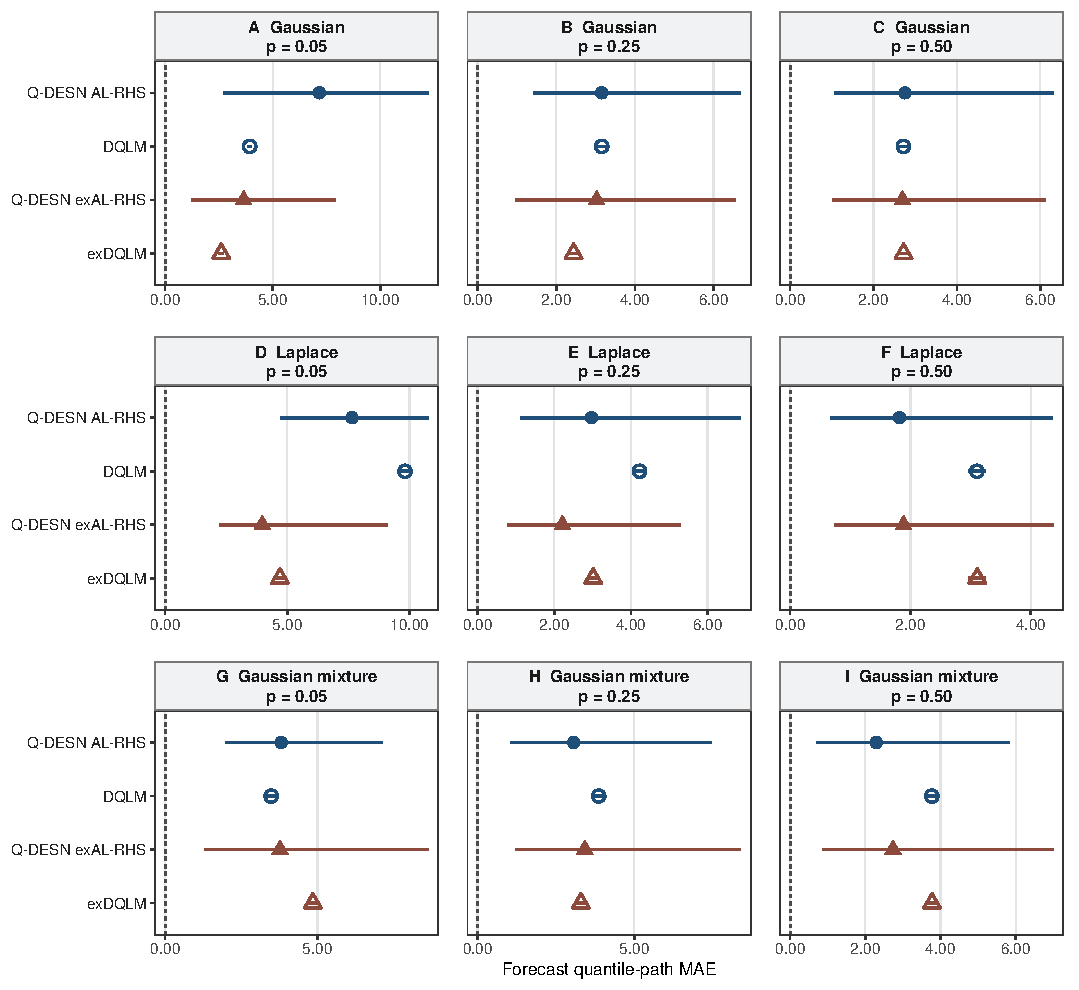
\includegraphics[width=0.98\textwidth]{figures/ch04-qdesn/independent_simulation/qdesn_validation_500obs_v14_mcmc_forecast_mae_intervals.pdf}
\caption[MCMC forecast criteria in the single-quantile simulation]{MCMC
forecast criteria in the single-quantile simulation, part I: quantile-path
mean absolute error (MAE). Points are posterior means and horizontal segments
are equal-tailed 95\% posterior intervals; lower values are better. Navy
circles identify the \(\AL\) models and muted-brick triangles the \(\exAL\)
models; filled symbols denote Q--DESN and open symbols the corresponding
dynamic quantile linear model. Panels A--I identify the data-generating family
and probability level and use separate horizontal scales. The dashed line
marks the exact data-generating-process value of zero. Intervals condition on
the simulated series, evaluation design, and case-specific selected
specification. Part II on the following page reports forecast check loss.}
\figalt{Nine panels compare posterior forecast-MAE means and 95 percent
intervals for four models across three innovation families and three
probability levels. Lower values are better.}
\label{qdesn:fig:simulation-500obs-mcmc-forecast-criteria-thesis}
\end{figure}

\begin{figure}[p]
\ContinuedFloat
\centering
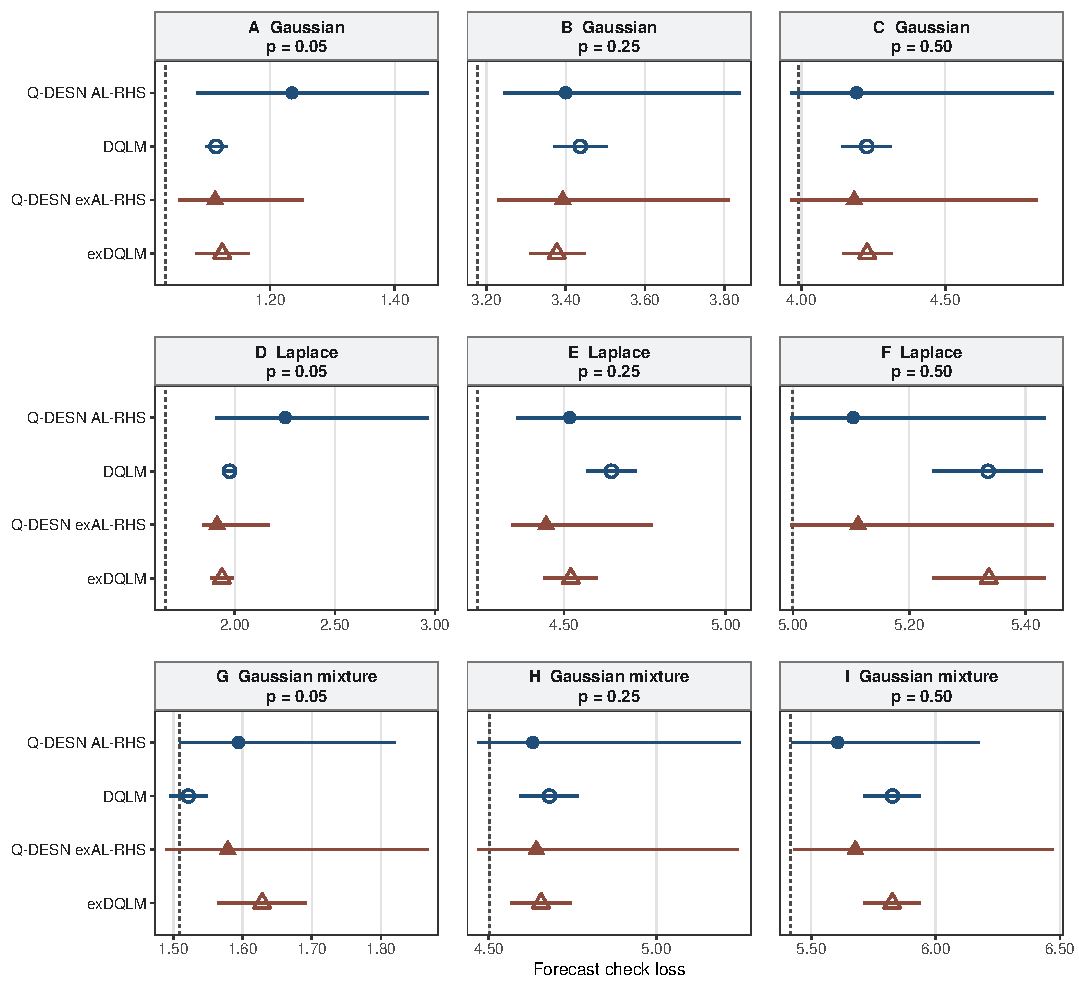
\includegraphics[width=0.98\textwidth]{figures/ch04-qdesn/independent_simulation/qdesn_validation_500obs_v14_mcmc_forecast_check_loss_intervals.pdf}
\caption*{Figure~\thefigure\ (continued), part II: MCMC forecast check loss.
Points are posterior means and horizontal segments are equal-tailed 95\%
posterior intervals; lower values are better. Model encodings and panels are
as in Figure~\ref{qdesn:fig:simulation-500obs-mcmc-forecast-criteria-thesis},
with separate horizontal scales. The dashed line marks the posterior mean
under the lowest-scoring model in each panel and is a visual reference.}
\figalt{Nine panels compare posterior forecast-check-loss means and 95 percent
intervals for four models across three innovation families and three
probability levels. Lower values are better.}
\end{figure}

\subsection{Joint multi-quantile study with a shared feature design}

The second simulation study compares joint and independent estimation at the
seven levels
\(p_k\in\{0.05,0.10,0.25,0.50,0.75,0.90,0.95\}\)
under the \(\AL\) and \(\exAL\) working likelihoods. Eight mechanisms span
Gaussian, Laplace, Gaussian-mixture, asymmetric-tail, persistent-heavy-tail,
Student-\(t\), regime-shift, and nonlinear dynamics. For each mechanism, one
DESN and RHS specification is selected using separate source realizations and
then shared by all four model classes. The 500-observation evaluation
realization is
not used for this selection. Thus differences among the 32 comparisons are
not confounded by model-specific feature maps or prior scales.

The evaluation fits use sequential initialization centered at the median.
A Gaussian ridge fit initializes Gaussian RHS--VB; the resulting compatible
estimates initialize the median \(\AL\) regression; and the remaining
independent \(\AL\) fits proceed toward the two tails. Each \(\exAL\) fit is
initialized from the \(\AL\) fit at the same level, the complete independent
grids initialize the corresponding joint fits, and each completed VB fit
initializes MCMC for the same model. These transfers determine starting values
only. Within each model cell, all five MCMC chains share fixed prior
hyperparameters and the same posterior target. The technical development gives the
complete calculation and chain allocation.

Held-out evaluation is sequentially conditional: regression coefficients and
reservoir weights remain fixed, while newly observed response lags enter later
forecast origins. Each comparison contains the same 990 origin--horizon rows.
The primary criterion is \(S_{\mathrm{DGP}}\) in
Eq.~\eqref{qdesn:eq:dgp-integrated-score-main}, computed for each retained MCMC draw
after monotone rearrangement. Independent quantile draws are combined by the
pre-specified chain-balanced product coupling described in the technical development.

Figure~\ref{qdesn:fig:joint-qdesn-corrected-v4-forecast-acrps} shows the corrected
posterior score comparison. Independent exQDESN has the smallest numerical
posterior mean in seven mechanisms; joint exQDESN is smallest for the Laplace
mechanism. The marginal intervals for the numerical winner and runner-up
overlap in every mechanism.
Of the 16 paired joint-minus-independent contrasts, four intervals favor
independent estimation and twelve include zero; none favors joint estimation.
The evidence therefore does not support a general forecast advantage from
joint estimation under this shared design.

\begin{figure}[!htbp]
\centering
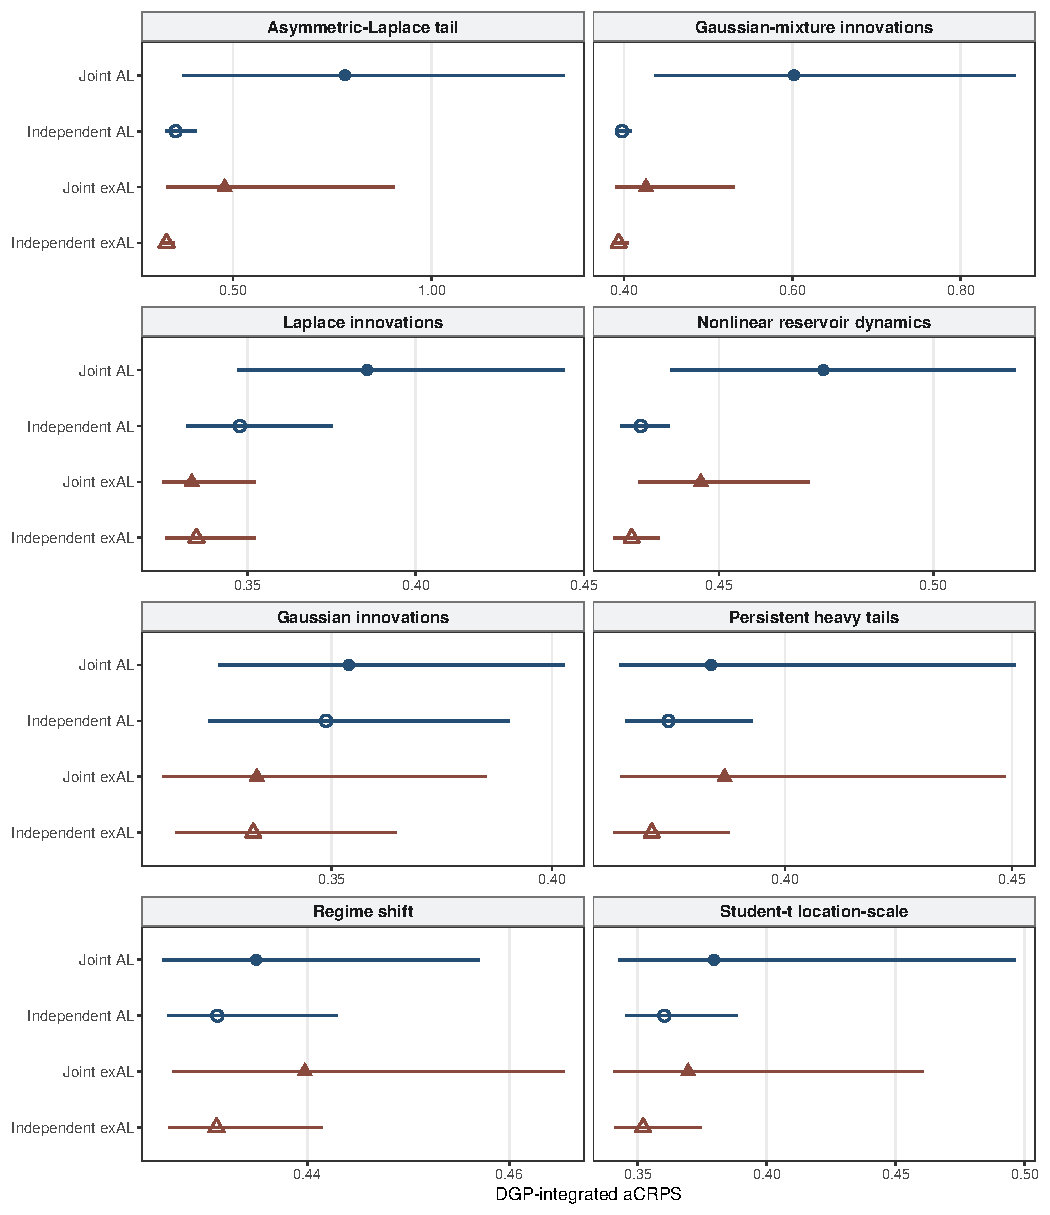
\includegraphics[width=0.94\textwidth]{figures/ch04-qdesn/joint_qdesn_simulation/joint_qdesn_corrected_v4_forecast_dgp_acrps.pdf}
\caption{Corrected posterior DGP-integrated \(\aCRPS\) for the joint multi-quantile study. Colored points are posterior means and horizontal segments are equal-tailed 95\% intervals. Lower values are better. Filled symbols denote joint fits, open symbols independent fits, blue \(\AL\), and red \(\exAL\). Marginal intervals for the numerical winner and runner-up overlap in every setting. Crossing frequencies and monotone-adjustment magnitudes are reported in the integrated technical material.}
\label{qdesn:fig:joint-qdesn-corrected-v4-forecast-acrps}
\end{figure}


Across the 47,520 adjacent-level forecast comparisons available to each model,
the raw crossing rates are 2.52\% for joint Q--DESN, 7.41\% for independent
Q--DESN, 0\% for joint exQDESN, and 0.57\% for independent exQDESN. These
percentages describe crossing frequency; the technical development reports the
corresponding mean and maximum absolute monotone adjustments to describe
magnitude. Joint exQDESN is therefore the most coherent raw specification in
this comparison, although its predictive score is not uniformly lowest.
Rearrangement produces ordered grids in all 32 comparisons. Posterior-score
diagnostics meet the pre-specified criteria in 22 comparisons and warrant
review in 10; all 16 \(\exAL\) scale--asymmetry assessments remain at review
level. Exact scores, fit recovery, crossing rates, and computational
diagnostics are reported in the technical development. A separate 50-replicate
variational analysis is retained as a sensitivity study.

\subsection{Simulation diagnostics and sensitivity}
\label{qdesn:sec:body-simulation-diagnostics}

The principal simulation comparisons are accompanied by posterior summaries,
multi-chain checks, and joint-quantile sensitivity analyses.  Those supporting
diagnostics are collected in Appendix~\ref{app:qdesn-technical}; they qualify
the empirical results but do not change the estimands or the reported primary
comparisons.

\section{GloFAS retrospective streamflow application}
\label{qdesn:sec:data}

\noindent\textbf{Retrospective case study.}
We consider one medium-range retrospective streamflow experiment using the
Global Flood Awareness System (GloFAS), which is jointly developed by the
European Commission and the European Centre for Medium-Range Weather Forecasts
and operated within the Copernicus Emergency Management Service
\citep{qdesn-AlfieriEtAl2013GloFAS,qdesn-CEMS2026GloFASDocumentation}.
GloFAS provides ensemble river-discharge forecasts for flood early warning and
verification \citep{qdesn-HarriganEtAl2023GloFASForecasts}. The analysis estimates
the conditional quantiles of a United States Geological Survey (USGS) gauge
record while using retrospective and issued GloFAS values to estimate a
time-varying discrepancy.

\subsection{Data and forecast-origin design}

Let \(T\) be the forecast origin, \(y_t=\log(y_t^{\mathrm{USGS}}+1)\) the
transformed gauge record through \(T\), \(g_t^{\mathrm{ret}}\) the transformed
retrospective GloFAS series, and \(g_{T+h,e}^{\mathrm{ens}}\) transformed
issued ensemble member \(e\) at horizon \(h\). The origin is
\GlofasApplicationCurrentOriginDate{}. The requested window contains 30 days,
from 26~December~2022 through 24~January~2023, but the issued GloFAS record
contains \GlofasApplicationCurrentScoredHorizons{} evaluable horizons through
22~January~2023. All 51 members are retained at each available horizon. Future
USGS values are excluded from fitting and used only for scoring. The
forecast-period precipitation and soil-moisture covariates are realized
PRISM/ERA5 values. The experiment is therefore a retrospective
oracle-covariate diagnostic, not a real-time forecast based only on information
available at \(T\).

\subsection{Application model}

\noindent\textbf{Latent-path discrepancy model.}
Two fixed DESN feature maps represent the reference process and the
GloFAS-minus-USGS discrepancy. For probability level \(p\), write
\(q_{p,t}=\vect x_t^{\mathrm{ref}\top}\vect\beta_p\) for the reference
quantile and \(d_{p,t}=\vect x_t^{\mathrm{disc}\top}\vect\delta_p\) for the
additive discrepancy. On the transformed scale, the historical and issued
working-likelihood contributions are
\begin{equation}
\begin{aligned}
\text{Reference history:}\quad
y_t\mid\cdot&\sim\AL_p(q_{p,t},\sigma_Y),\\
\text{Retrospective GloFAS:}\quad
g_t^{\mathrm{ret}}\mid\cdot&\sim\AL_p(q_{p,t}+d_{p,t},\sigma_G),\\
\text{Issued member:}\quad
g_{T+h,e}^{\mathrm{ens}}\mid\cdot&\sim
\AL_p(q_{p,T+h}+d_{p,T+h},\sigma_G).
\end{aligned}
\label{qdesn:eq:glofas-part4-main}
\end{equation}
The unavailable path \(y_{T+1:T+30}\) is represented as latent during fitting
and recursively supplies future response lags to the reference reservoir. Each
of the 51 issued members has weight \(1/51\), so every issued horizon has total
weight one. This weighting is applied to the augmented complete-data working
likelihood.

The reported model estimates the seven levels \(0.05\), \(0.20\), \(0.35\),
\(0.50\), \(0.65\), \(0.80\), and \(0.95\) jointly by VB, with AL working
likelihoods and adjacent-quantile RHS shrinkage for the reference and
discrepancy coefficient paths. No crossing correction is applied; the selected
issued-window grid has no crossings. The technical development gives the source weighting,
reservoir specifications, latent-path approximation, and convergence record.

\subsection{Retrospective application results}

The selected Joint AL estimate completed ten outer sweeps. All inner fits and
RHS release conditions were satisfied, and all 14 reference and discrepancy
RHS blocks changed after release. Its final maximum parameter change was
\(0.004154\), above the pre-specified \(0.001\) outer tolerance. We therefore
describe it as cap-stabilized after RHS release, not as strictly
outer-converged. No MCMC application fit is reported.

\noindent\textbf{Forecast-period scores.}
Table~\ref{qdesn:tab:glofas-application-score} compares the selected Joint AL model
with the completed independent quantile regressions, two Gaussian predictive
baselines, and raw GloFAS. Joint AL reduces \(\aCRPS\) from
\GlofasApplicationCurrentRawAcrps{} for raw GloFAS to
\GlofasApplicationCurrentQdesnAcrps{}, a
\GlofasApplicationCurrentAcrpsReduction{} reduction, and has the smallest mean
check loss and interval score among the quantile-regression models. Independent
AL gives similar scores and the same empirical 90\% coverage of \(0.929\).
Independent exAL has larger scores and lower coverage in this forecast window.

The Normal Ridge baseline has the smallest numerical \(\aCRPS\), \(0.8062\),
but its empirical 90\% coverage is \(0.250\) and its interval score is
\(13.8539\), compared with \(0.929\) and \(5.3889\) for Joint AL. This
difference illustrates that the summaries answer distinct questions: mean
check loss weights the seven levels equally, whereas \(\aCRPS\) uses the
trapezoidal weights in Eq.~\eqref{qdesn:eq:acrps-main}, and interval score and
coverage assess the central forecast interval. The comparisons are descriptive
for one forecast origin; no sampling-uncertainty calculation for score
differences is available.

This issued-window improvement does not extend to the historical fit. On the
common six-level grid, the Part 4 Joint AL \(\aCRPS\) is 68.6\% larger than FR09 over
the full history and is 104.2\%, 51.4\%, and 8.6\% larger over the final 1000,
200, and 50 dates, respectively. FR09 is therefore retained as the stronger
historical benchmark, while Part 4 is interpreted only for this single-origin
issued-window experiment.

Figure~\ref{qdesn:fig:glofas-application-forecast-period} places the reported
quantile paths against the observed history, held-out gauge record, and issued
GloFAS ensemble over the single forecast window.

\begin{table}[!htbp]
\centering
\TableStyle
\caption{Forecast scoring for the GloFAS retrospective analysis at origin
\GlofasApplicationCurrentOriginDate{}. Scores use the 28 issued horizons and
are computed on the \(\log(\mathrm{USGS}+1)\) scale and the common probability
grid \(0.05,0.20,0.35,0.50,0.65,0.80,0.95\). Mean check loss averages the
seven level-specific losses equally, whereas \(\aCRPS\) uses the trapezoidal
weights in Eq.~\eqref{qdesn:eq:acrps-main}. The Normal rows summarize Gaussian
predictive distributions on the same dates and probability grid. Lower scores
are better. Coverage is empirical coverage of the nominal 90\% interval; the
final column gives the \(\aCRPS\) reduction relative to raw GloFAS.}
\label{qdesn:tab:glofas-application-score}
\input{\GlofasApplicationCurrentScoreTable}
\end{table}

\begin{figure}[!htbp]
\centering
\includegraphics[width=0.94\textwidth]{\GlofasApplicationCurrentForecastWindowFigure}
\caption{Joint AL Q--DESN latent-path analysis over the final 30 historical
dates and 28 issued GloFAS horizons. The seven probability levels share a
single-blue scale that darkens toward both tails; historical quantile paths
are dashed and issued paths are solid. Forest-green filled circles joined by a
thin solid line denote USGS observations available through the origin.
Forest-green open circles joined by a short-dashed line denote the withheld
USGS values used only for scoring.
Dark-orange lines show retrospective GloFAS and the 51 issued ensemble members.
The lower panel gives the corresponding GloFAS-minus-USGS discrepancy paths.
The vertical dotted line marks the forecast origin. No crossing correction is
applied. All values are on the transformed scale.}
\figalt{Two panels show the seven Joint AL Q--DESN quantile paths over 30
historical dates and 28 forecast dates. The upper panel contrasts observed and
withheld USGS values with retrospective and issued GloFAS values. The lower
panel shows fitted and observed GloFAS-minus-USGS discrepancies. Historical
quantile paths are dashed, forecast paths are solid, and a vertical line marks
the forecast origin.}
\label{qdesn:fig:glofas-application-forecast-period}
\end{figure}

\subsection{Latent-path ensemble interpretation}
\label{qdesn:sec:body-latent-path}

The GloFAS ensemble experiment uses a latent-path augmented working likelihood
to connect ensemble members to the observed streamflow target.  The reported
comparison is conditional on that construction and its numerical
approximation.  Appendix~\ref{app:qdesn-technical} gives the full augmented
model and sensitivity evidence.

\section{Region-frozen PriceFM application}
\label{qdesn:sec:pricefm-application}

The second application compares Q--DESN day-ahead electricity-price forecasts
with version~4 of PriceFM \citep{qdesn-YuEtAl2026PriceFM}. The release covers
European bidding regions at 15-minute resolution from 1~January~2022 through
1~January~2026 and includes price, load, solar, and wind forecasts. Average
quantile loss (AQL) is evaluated on the PriceFM probability grid at matched
held-out timestamps for 114 region--fold comparisons.

\subsection{Comparison design}

The comparison contains \PricefmFullRegionFolds{} region--fold evaluations,
spanning \PricefmFullRegions{} European bidding regions and
\PricefmFullFolds{} rolling folds. For each region, one Q--DESN specification
was selected using training and validation data, then frozen before the test
scores were examined. The reservoir specification, RHS global scale, feature
set, and working-likelihood family are therefore common to the three folds of
that region. The selected specifications use AL in \PricefmCurrentAlRegions{}
regions and exAL in \PricefmCurrentExalRegions{} regions. There were no post-test
changes and no substitutions from the earlier case-specific comparison.

Each evaluation is scored on the fold-aligned held-out timestamps and
probability levels \PricefmFullPaperQuantiles. Throughout this section,
\(\Delta\) AQL denotes Q--DESN AQL minus PriceFM AQL. Negative values indicate
lower Q--DESN AQL; positive values indicate lower PriceFM AQL.

\noindent\textbf{Information set.}
The model-selection rule is prospective with respect to the held-out test
scores, but the covariate comparison remains retrospective. The Q--DESN
specifications use retrospectively observed own-region load, solar, and wind
lead covariates; selected neighborhood feature sets additionally use
retrospectively observed neighboring-region summaries. The results therefore
assess a test-separated retrospective comparison rather than real-time
electricity-price forecasting.

\subsection{Results}

Across the aligned benchmark, Q--DESN has lower AQL in
\PricefmFullQdesnWins{} of \PricefmFullRegionFolds{} region--fold evaluations
(\PricefmFullQdesnWinRate{}), while PriceFM has lower AQL in
\PricefmFullPricefmWins{}. The mean Q--DESN AQL is
\PricefmFullMeanQdesnAql{}, compared with \PricefmFullMeanPricefmAql{} for
PriceFM, giving mean \(\Delta\) AQL \PricefmFullMeanDeltaAql{} and median
\(\Delta\) AQL \PricefmFullMedianDeltaAql{}. Thus, under the prospectively
frozen region-level specifications, Q--DESN has slightly higher aggregate AQL.
When scores are first averaged within region, Q--DESN is lower in
\PricefmCurrentRegionWins{} of \PricefmFullRegions{} regions and PriceFM is lower
in \PricefmCurrentRegionLosses{}.

\begin{table}[!htbp]
\centering
\caption{PriceFM-aligned test comparison under the region-frozen Q--DESN
protocol. Entries are unweighted summaries across region--fold evaluations,
overall and by fold. The Q--DESN specification for each region was selected
using training and validation data and held fixed across its three test folds.
Here \(\Delta\) AQL is Q--DESN minus PriceFM, so negative values favor Q--DESN.
AQL is in EUR/MWh; all scores use matched held-out timestamps and the same
seven probability levels.}
\label{qdesn:tab:pricefm-matched-aql-comparison}
\begingroup
\TableStyle
\scriptsize
\setlength{\tabcolsep}{3pt}
\begin{tabular}{@{}lrrrrrrr@{}}
\toprule
Comparison set & $n$ & \shortstack{Q--DESN\\lower} & \shortstack{PriceFM\\lower} & \shortstack{Mean\\Q--DESN AQL} & \shortstack{Mean\\PriceFM AQL} & \shortstack{Mean\\$\Delta$} & \shortstack{Median\\$\Delta$} \\
\midrule
Overall & 114 & 54 & 60 & 7.217 & 7.039 & 0.178 & 0.071 \\
Fold 1 & 38 & 18 & 20 & 7.353 & 7.297 & 0.056 & 0.084 \\
Fold 2 & 38 & 24 & 14 & 6.799 & 6.826 & -0.027 & -0.155 \\
Fold 3 & 38 & 12 & 26 & 7.499 & 6.993 & 0.506 & 0.247 \\
\bottomrule
\end{tabular}
\endgroup

\end{table}

The fold summaries show a small Q--DESN advantage in fold~2
(mean \(\Delta=-0.027\)), a small PriceFM advantage in fold~1
(\(0.056\)), and a larger PriceFM advantage in fold~3 (\(0.506\)). Region-level
differences are also heterogeneous; the technical development displays all 38 region
means. The earlier R92 surface has lower mean Q--DESN AQL
(\PricefmCurrentHistoricalAql{}) but used a case-specific, held-out-informed
selection rule. It is retained only as historical sensitivity evidence and is
not combined with R98. A complete R98 forecast-lead table was not available,
so the earlier 72-case horizon summary is not presented as part of this
114-case comparison.

% ============================================================

\subsection{Regional and historical sensitivity}
\label{qdesn:sec:body-pricefm-sensitivity}

The region-frozen comparison is not uniform across regions or historical
windows.  Appendix~\ref{app:qdesn-technical} preserves the detailed
heterogeneity and sensitivity evidence; the discussion below retains the
resulting limitations on generalization.

\section{Chapter discussion}
\label{qdesn:sec:discussion}

Q--DESN treats the fixed DESN reservoir as a nonlinear feature map and places
Bayesian quantile inference on the regression coefficients. Posterior
simulation and variational inference concern the regression, likelihood, and
shrinkage parameters conditional on the fixed reservoir features. The empirical
results evaluate this conditional Bayesian quantile-regression analysis under
specified reservoir constructions.

The AL and exAL families are used as working likelihoods for conditional
quantiles. They provide posterior distributions and conditionally tractable
augmented updates. The
simulation and application sections report fit recovery, forecast scoring,
empirical predictive coverage, monotonicity, and convergence diagnostics to
assess the model-based summaries under possible misspecification. Sandwich
corrections and generalized-Bayes calibration for composite quantile
likelihoods remain important topics for further study.

The multi-quantile construction makes the same distinction. Independent
single-level Q--DESN fits followed by isotonic regression or rearrangement
produce monotone quantile curves from level-wise regressions. The joint
quantile-vector extension shares information across quantile levels through RHS
shrinkage on adjacent coefficient differences. This shrinkage can reduce
crossings but does not enforce monotonicity. Ordered parameterizations or
monotone rearrangement can be used when monotonicity is required.

The single-quantile dynamic simulations assess recovery and held-out
forecasting under known data-generating mechanisms. The joint multi-quantile
study assesses quantile-path recovery and crossings under known conditional
quantile paths. The single-quantile study uses one reproducible dynamic root
for each family and quantile level and conditions on a selected reservoir
realization; its posterior intervals do not measure repeated-data-set or
reservoir-seed variability. The available MCMC and VB--LD summaries also use
separately selected specifications in several single-level comparisons, so
they do not provide a controlled estimate of VB--LD approximation error. The
balanced joint study uses MCMC as its primary confirmation layer, while
VB--LD supplies screening and initialization evidence.

The GloFAS application studies one retrospective
oracle-covariate origin with a joint AL--RHS VB latent-path model. Its
issued-window grid required no crossing correction and had empirical 90\%
coverage of 0.929 over 28 issued horizons, but the estimate reached its
iteration cap before the strict outer tolerance and had poorer historical
\(\aCRPS\) than FR09. The PriceFM
comparison uses one training- and validation-selected Q--DESN specification
per region, frozen across three held-out folds. Its aggregate AQL is slightly
higher than that of the matched PriceFM forecasts, with differences that vary
by fold and region. The covariates include retrospectively observed leads, so broader
rankings of Q--DESN against dynamic quantile or foundation-model alternatives
require evaluations across additional data sets, forecast origins, and
reservoir specifications.

Several extensions are natural. On the statistical side, future work should
study calibrated composite-likelihood scaling, hard or probabilistic
non-crossing constraints, richer covariance structures for quantile
differences, and sensitivity to reservoir scaling on bounded feature domains.
On the computational side, the joint model calls for sparse precision solvers,
targeted covariance extraction for VB, and diagnostics comparing VB with
MCMC on small joint problems. On the application side, multi-origin operational
GloFAS studies with covariates known at the forecast origin, paired PriceFM
uncertainty analyses, and explicitly joint PriceFM analyses are needed before the joint
quantile-vector prior can be interpreted in an application-level benchmark.

Q--DESN combines fixed nonlinear recurrent features with Bayesian regression
for dynamic conditional quantiles. The results document conditional-quantile
estimation under the specified simulation designs and retrospective
applications and identify the settings requiring broader validation.

% ============================================================
